\tikzstyle{block} = [rectangle, draw, fill=white, 
    text width=6em, text centered, minimum height=4em]
\tikzstyle{description}=[above,color=black]
\tikzstyle{line} = [draw, -latex]

\resizebox{\textwidth}{5cm}{
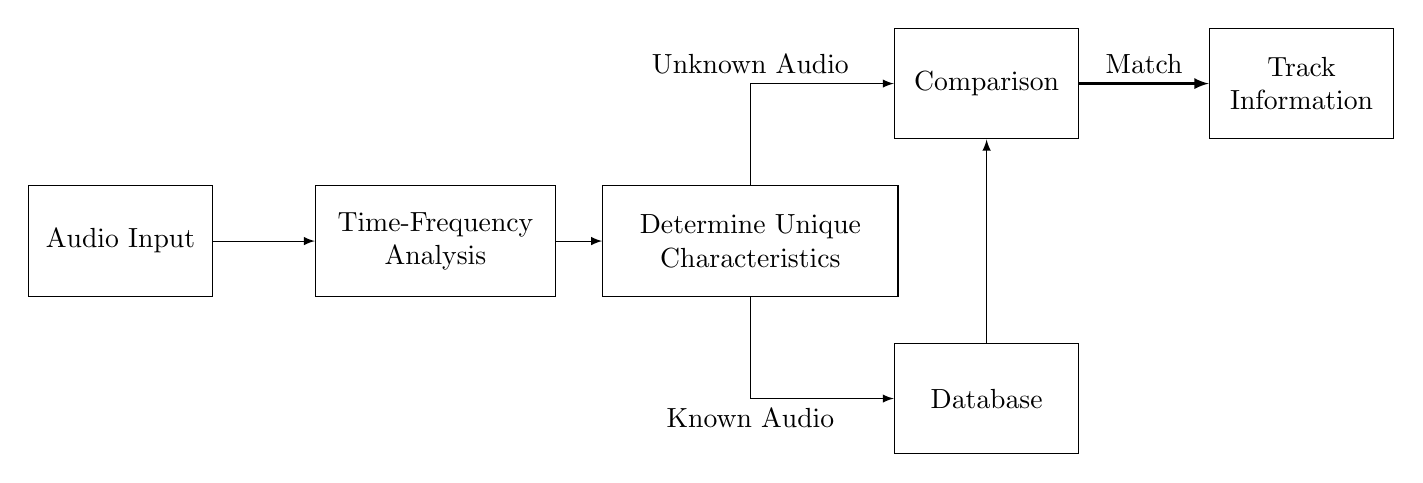
\begin{tikzpicture}[node distance =4cm, auto]
\node (AudioInput) [block]{Audio Input};
\node (TimeFreq) [block, right of=AudioInput,text width=8em]{Time-Frequency Analysis};


\node (PCA) [block, right of=TimeFreq, text width=10em]{Determine Unique Characteristics};


\coordinate [right of=PCA, node distance=3cm](T1);
%Above
\node (Comparison)[block, above of=T1, node distance=2cm]{Comparison};
\node (TrackInfo)[block, right of=Comparison]{Track Information};

%Below
\node (Database)[block, below of=T1, node distance=2cm]{Database};


\path [line](AudioInput)--(TimeFreq);
\path [line](TimeFreq)--(PCA);

\path [line](PCA)|-node[description, above]{Unknown Audio}(Comparison);
\path [line,thick](Comparison)--node[description, above]{Match}(TrackInfo);
\path [line](PCA)|-node[description, below]{Known Audio}(Database);
\path [line](Database)--(Comparison);

\end{tikzpicture}}